% !TEX root = ../thesis-example.tex
%
\chapter{Metodología}
\label{Metodologia}

En este capítulo se presenta el método y algoritmos desarrollados para cálculo de la entropía en mercados financieros.
La metodología presentada tiene como objetivo ayudar a detectar si un mercado es \textit{estable} en el tiempo a partir de la entropía calculada.
Adicionalmente, el método propuesto puede ser utilizado para detectar momentos (fechas) en los que la entropía es mínima. 
Esto se traduce como un intervalo de tiempo en el que el precio no cambia significativamente.


\section{Algoritmo para el calculo de entropia simple}
\label{sec_algorithm}
La metodología implementada para el cálculo de la entropía así como el procesamiento de datos se presenta en el diagrama \ref{diagramaentropia1}.


\begin{figure}[h]
	\centering
	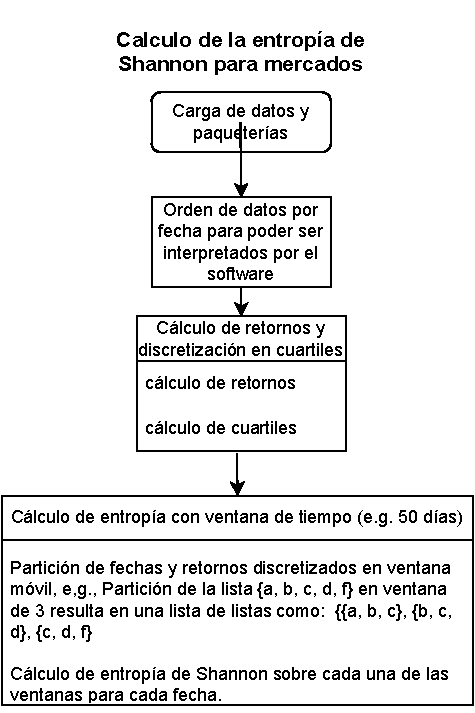
\includegraphics[width=0.7\linewidth]{figures/diagrama_entropia1}
	\caption{Diagrama del algoritmo utilizado para el c\'alculo de entrop\'ia de Shannon en mercados financieros.}
	\label{diagramaentropia1}
\end{figure}

En este diagrama se identifican cuatro etapas principales:

\begin{itemize}
	\item Carga de datos
	\item Pre-procesamiento de datos
	\item Cálculo de retornos y cuartiles o cuantiles
	\item Cálculo de entropía
\end{itemize}

Los algoritmos presentados en esta Tesis fueron desarrollados en el lenguage de programación Wolfram Mathematica y Matlab.


\subsection{Procesamiento de datos de precios de mercados}
\label{sec_data}
Los precios de los mercados utilizados en esta Tesis fueron obtenidos del portal Yahoo Finance. 
Cabe mencionar que los precios son registrados cada 24 horas excepto los días sábado y domingo. También es importante mencionar que un año en el mercado de valores generalmente incluye 252 días, esto debido a que se presentan días en que se conmemora algo importante como lo es el día de año nuevo, el día de Martin Luther King, el día de la independencia, entre otros. 

Se descargaron las datos de precios entre DD/MM/YYYY y DD/MM/YYYY de los mercados Dow Jones Industrial Average (DWJ), Índice BMV IPC (IPC), \textit{Deutscher Aktienindex} (DAX), y la bolsa de valores de Tokio Nikkei 225 (Nikkei).

Un ejemplo de la base de datos de precios descargada se presenta en la tabla \ref{ejemplo_data}.
\begin{table}[]
	\begin{tabular}{|l|l|}
		\hline
		Fechas         & Precios \\ \hline
		Vi 8-11-1991   & 1606.2  \\ \hline
		Lu 11-Nov-1991 & 1609    \\ \hline
		Ma 12-Nov-1991 & 1621.2  \\ \hline
		Mi 13-Nov-1991 & 1623.2  \\ \hline
		Ju 14-Nov-1991 & 1621    \\ \hline
		Vi 15-Nov-1991 & 1629.4  \\ \hline
		Lu 18-Nov-1991 & 1611.9  \\ \hline
		Ma 19-Nov-1991 & 1599.1  \\ \hline
		Ju 21-Nov-1991 & 1598.1  \\ \hline
		Vi 22-Nov-1991 & 1600.3  \\ \hline
		Lu 25-Nov-1991 & 1589.2  \\ \hline
		Ma 26-Nov-1991 & 1602.9  \\ \hline
		Mi 27-Nov-1991 & 1586.2  \\ \hline
		Ju 28-Nov-1991 & 1588.2  \\ \hline
		Vi 29-Nov-1991 & 1566.6  \\ \hline
	\end{tabular}
\label{fechasdatabase1}
\caption{Primeras 15 fechas de la base de datos correspondiente a Dow Jones.}
\end{table}

Las columnas de la base de datos corresponden a la fecha en la que se realizó el registro de precio respectivo.
Las bases de datos de cada uno de los mercados fueron depuradas y ordenadas. Esta depuración corresponde a identificar y eliminar las fechas en las que no hay precio registrado para evitar errores de cálculo.

\begin{table}
\begin{center}
\begin{tabular}{|c|c|}
	\hline 
	Fecha & precio \\ 
	\hline 
	DD/MM/YYYY & $$$$ \\ 
	DD/MM/YYYY & $$$$ \\ 
	DD/MM/YYYY & $$$$ \\ 
	\hline 
\end{tabular} 
	\label{ejemplo_data}
	\caption{Ejemplo de base de datos de mercados financieros.}
\end{center}
\end{table}

\subsection{Cálculo de retornos de precios de mercados}
\label{sec_retornos}
Luego que se han cargado los datos, y se han ordenado es necesario calcular los retornos de los precios. 
%y ello conlleva a que no va a haber una media central en los datos. 
Los retornos permiten analizar fácilmente la tasa de cambio en el tiempo.
En esta Tesis se eligió trabajar con los retornos de los precios y no con los precios directamente debido a las propiedades de los retornos presentadas en la subseccion \ref{retornos}.
Aunque los retornos son una mejor representación de los precios, aún presentan picos que sobresalen de la media. 
%La estandarización permite destacar los retornos que realmente son relevantes. 
%%%-----NO SE APLICO ESTANDARIZACION NO ?????
%Ya que cada retorno ha sido estandarizado con su respectiva fecha,  
Posteriormente se procede a discretizar los retornos mediante un proceso que divide en Q quantiles a los retornos.
Por ejemplo, la Tabla \ref{quantile_example} muestra un ejemplo de discretizacion de los retornos en cuatro cuartiles. 
En este ejemplo a cada cuartil se le asigna la etiqueta 1, 2, 3, 4 dependiendo del intervalo al que corresponde el valor de retorno.
De este modo, la Tabla \ref{ejemplo_data-returns} muestra un ejemplo de etiquetado para los retornos calculados sobre una base de datos.

\begin{table}	
\begin{center}
	\begin{tabular}{ |r | l | c| }
		\hline
		Cuartiles &  Valor de retorno & Etiqueta  \\ \hline
		Primer cuartil & $(-\infty , Q_2)$ & 1 \\
		Segundo cuartil & $[Q_2 , Q_3)$   & 2\\ 
		Tercer cuartil &  $[Q_3 , Q_4)$   & 3 \\
		Cuarto cuartil & $[Q_4 , \infty)$ &4\\ 
		\hline
	\end{tabular}
	\label{quantile_example}
		\caption{Intervalos de cuartiles y etiquetas aplicadas a los retornos.}
\end{center}
\end{table}


\begin{table}
	\begin{center}
	\begin{tabular}{|c|c|c|}
		\hline 
		Fecha & retorno & cuartil \\ 
		\hline 
		DD/MM/YYYY & $$$$ & 1\\ 
		DD/MM/YYYY & $$$$ & 2\\ 
		DD/MM/YYYY & $$$$ & 4\\ 
		\hline 
	\end{tabular} 
	\label{ejemplo_data-returns}
	\caption{Ejemplo de etiquetado para una base de datos de mercados financieros.}
\end{center}
\end{table}

\subsection{Cálculo de la entropia}
\label{sec_entropia}
El cálculo de la entropía se realizó de acuerdo a la ecuación de Shannon \ref{entropySha}.
Para poder calcular la entropía se calculó la probabilidad de cada etiqueta sobre intervalos de tiempo deslizantes de $\Delta t_{ent})$.
Los retornos y etiquetas fueron calculados y asignados como se explico en la sección anterior. 
Con los intervalos dados por los cuartiles y la discretización de los retornos se obtiene todo lo necesario para calcular la entropía.
La ventana de tiempo deslizante para el cálculo de la entropía se corresponde a subconjuntos de datos agrupados en listas de N elementos.
En la Tabla \ref{entropytable} se muestra un ejemplo de la entropía calculada para un conjunto de datos. 
La ventana deslizante aplicada para el cálculo de entropía en este ejemplo es de 50 dias.

\begin{table}
	\begin{center}
	\begin{tabular}{|c|c|c|}
		\hline 
		Fecha & retorno & entropia \\ 
		\hline 
		DD/MM/YYYY & $$$$ & N entropia\\ 
		DD/MM/YYYY & $$$$ & N entropia\\ 
		DD/MM/YYYY & $$$$ & N entropia\\ 
		\hline 
	\end{tabular} 
	\label{entropytable}
	\caption{Ejemplo de entropía calculada para una base de datos de mercados financieros.}
\end{center}
\end{table}




\section{Cálculo de entropía con retornos de medias móviles}
\label{metodo_MAV}
El método explicado en la sección anterior ahora es estudiado con una modificación en el cálculo de retornos.
Dicha modificación consiste en el cálculo de la media del precio sobre una ventana deslizante de tiempo $\Delta t_{MAV})$(i.e., media móvil) (ver Figura \ref{entropiamav}). 
El intervalo de la ventana deslizante impacta directamente la curva de precios.
De este modo se observa que una ventana deslizante grande (e.g. 50 dias) ver Figura \ref{mav50Entropy10nq23} tiene un efecto de suavizado de la curva mas claro que una ventana corta (e.g., 10 dias) ver Figura \ref{mav10Entropy10nq23} lo que permite observar una diferente cantidad diferente de picos en los valores mínimos de entropía en ambos casos. 



\begin{figure}[h]
	\centering
	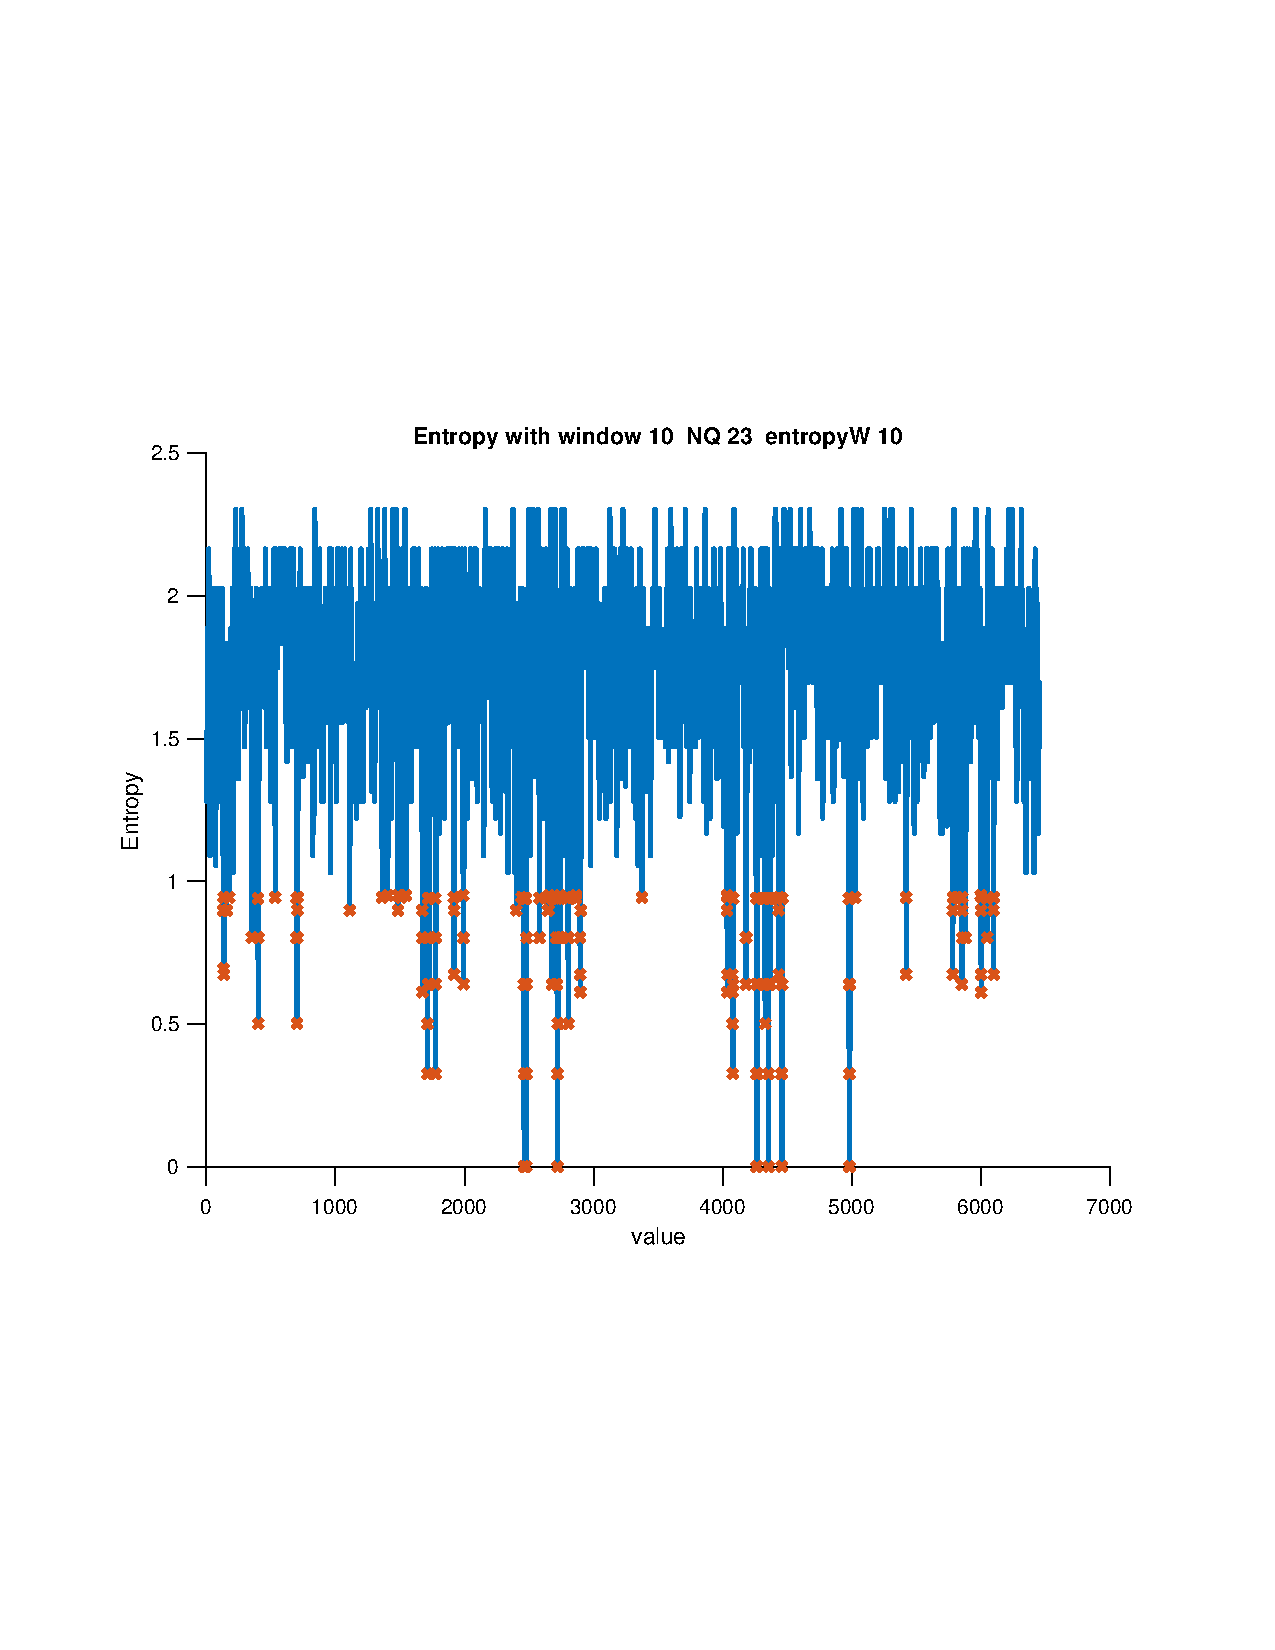
\includegraphics[width=0.7\linewidth]{figures_matlab/Entropy_window_10_NQ_23_entropyW_10}
	\caption{Valores de entropía con filtro de media móvil de 10 días y agrupación de 10 en 10 para la entropía de Shannon en el caso de 23 cuantiles el mercado DJJA.}
	\label{mav10Entropy10nq23}
\end{figure}

\begin{figure}[h]
	\centering
	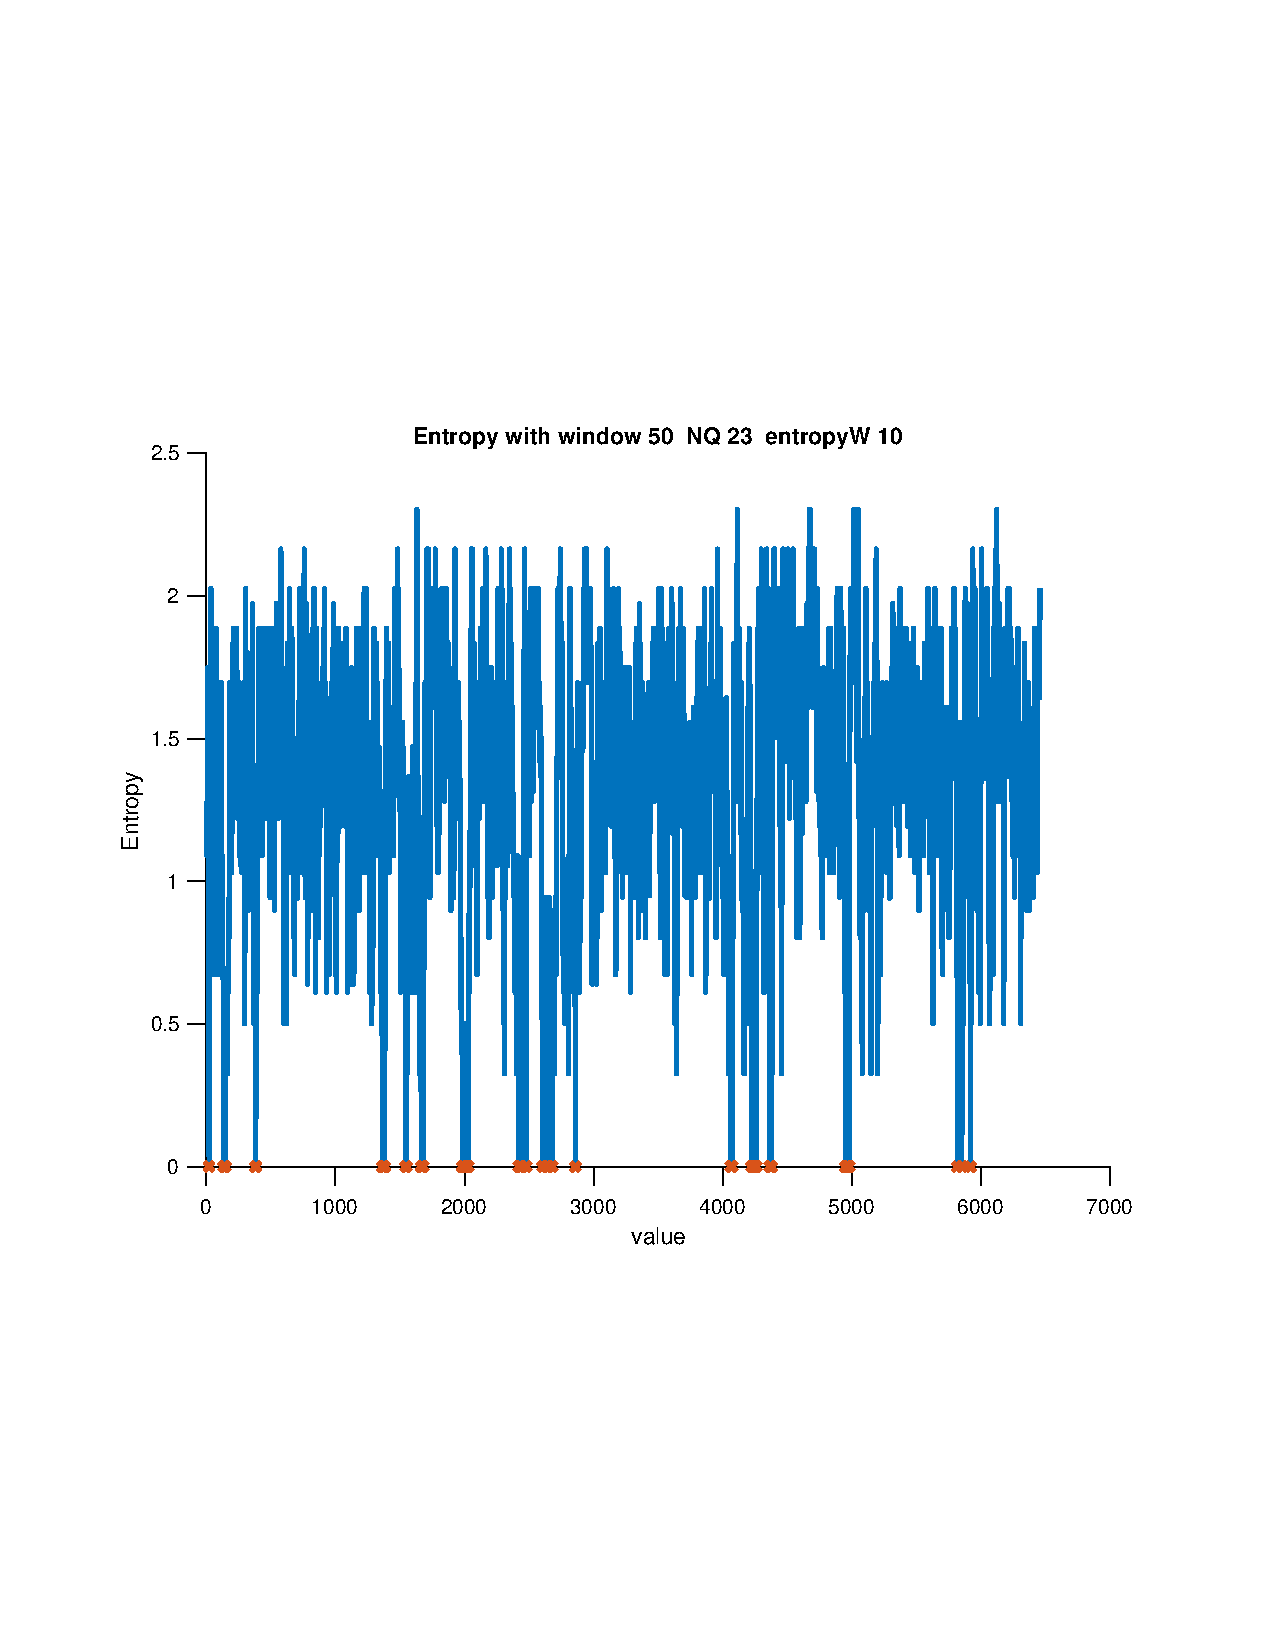
\includegraphics[width=0.7\linewidth]{figures_matlab/Entropy_window_50_NQ_23_entropyW_10}
	\caption{Valores de entropía con filtro de media móvil de 50 días y agrupación de 10 en 10 para la entropía de Shannon en el caso de 23 cuantiles el mercado DJJA.}
	\label{mav50Entropy10nq23}
\end{figure}


Una vez que las medias móviles de precio son calculadas, se calculan los retornos tal como en la Ecuacion \ref{retornos}.
Después se aplica el método descrito en la Sección \ref{sec_entropia} para calcular la entropía.
Las observaciones así como conclusiones respecto a la aplicación de medias móviles serán discutidas en profundidad en la sección \ref{Conclusiones}.


\begin{figure}
	\centering
	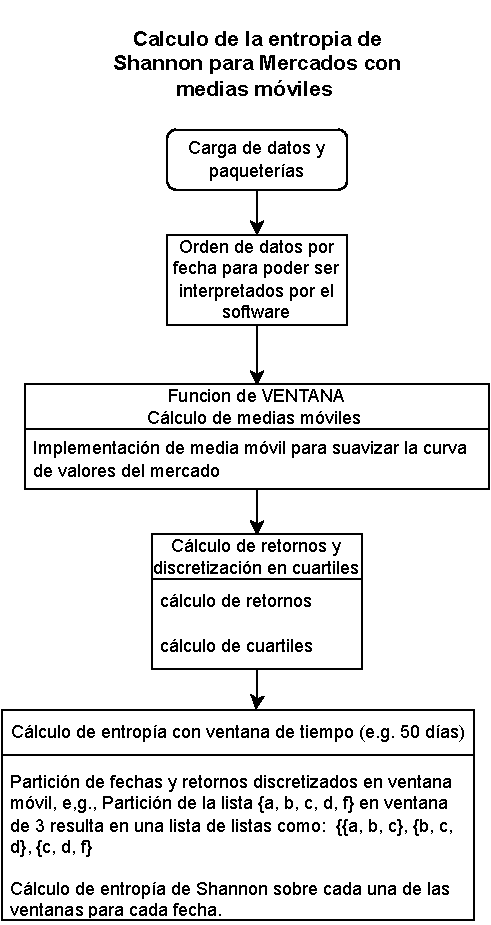
\includegraphics[width=0.7\linewidth]{figures/entropiaMAV}
	\caption{Diagrama del algoritmo utilizado para el c\'alculo de entrop\'ia de Shannon en mercados financieros con medias m\'oviles.}
	\label{entropiamav}
\end{figure}



\section{Simulación de un mercado eficiente}

Para fines de comparación y validación de la metodología propuesta en las secciones previas a mercados financieros reales se realizó una simulación de un mercado eficiente.
Esta simulación utiliza los datos del mercado real para calcular la media y desviación estándar  de los retornos (no estandarizados) de los precios reales. 
Posteriormente se obtienen retornos simulados a los cuales se les asigna una fecha.

A partir de este punto se realizaron dos simulaciones que se pueden apreciar en el diagrama \ref{simulacion}.
La primera es que a dichos retornos simulados se les aplica el proceso para el cálculo de entropía de la figura \ref{diagramaentropia1}.
En la segunda se aplica el proceso de medias móviles como se presenta en \ref{entropiamav}.

\begin{figure}
	\centering
	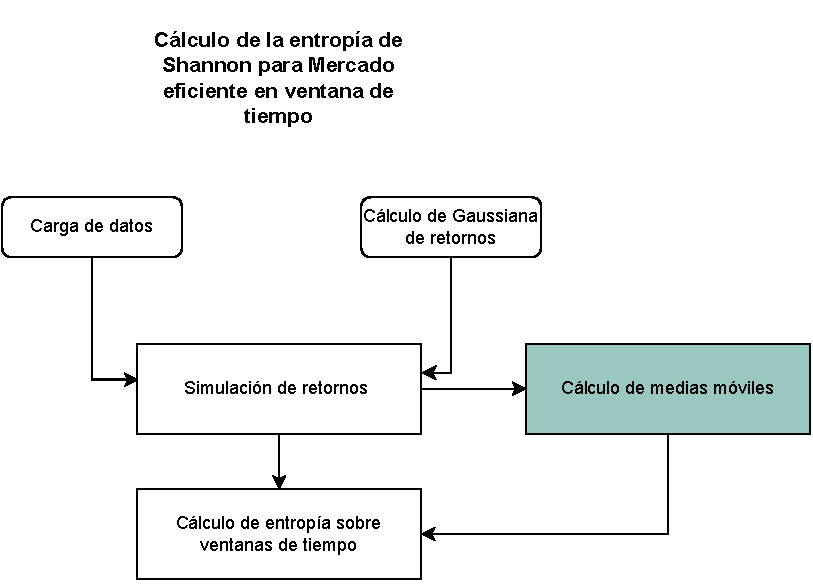
\includegraphics[width=0.9\linewidth]{figures/simulacion}
	\caption{Diagrama del algoritmo de calculo de entropia para la simulacion de mercado eficiente. }
	\label{simulacion}
\end{figure}

La simulación del mercado eficiente proporciona la forma en que puede ser utilizada para calcular un umbral que permita seleccionar los valores de entropía mínima en los mercados reales. 
 
\section{Ajuste de distribuciones estadísticas}
\label{ajuste}
Para poder seleccionar los valores de mínima entropía se aplicó un ajuste de distribuciones estadísticas a los valores de entropía.
Este ajuste es realizado utilizando el paquete \textit{Distribution Fitter} de Matlab.
Este paquete está compuesto de una aplicación que permite ajustar de manera interactiva funciones de probabilidad.
Las funciones de ajuste pueden también ser utlizadas fuera del ambiente interactivo.

Las distribuciones que serán ajustadas son:

\begin{itemize}
	\item Normal
	\item Poisson
	\item ttt
	\item ttt
	\item ttt
\end{itemize}


Por otro lado, se aplicaron diferentes test para ajustar una distribución normal a los valores de entropía calculados.
\begin{itemize}
	\item Cramér-von Mises
	\item Kolmogorov-Smirnov
	\item Pearson $X^2$
	\item Anderson-Darling
	\item Watson $U^2$
\end{itemize}



\section{Búsqueda de mínimos de entropía}

Uno de los objetivos de esta Tesis es buscar un método que permita la identificación de mínimos de entropía en los mercados financieros.
Sin embargo, en la metodología descrita en la Sección \ref{metodo_MAV} se observa que existen tres parámetros dados por el usuario:
\begin{itemize}
	\item la talla de ventana deslizante $\Delta t_{MAV}$ para suavizado de la curva de precios,
	\item la talla de ventana deslizante $\Delta t_{ent}$ para el cálculo de la entropía y
	\item el número de cuantiles $Q$ sobre los cuales se calcula la entropía de Shannon.
\end{itemize}

Estos parámetros actúan directamente sobre el cálculo de la entropía de la siguiente manera: 
el valor de $\Delta t_{MAV})$ tiene un impacto directo sobre el suavizado de la curva de precios, y como consecuencia, sobre la determinación de los valores de entropía. 
$\Delta t_{ent}$ tiene un impacto en el número de muestras utilizadas en el cálculo de la entropía, este valor impacta directamente el valor de la probabilidad de los valores de $Q$. 
Por otro lado, el valor de $Q$ es el número de categorías utilizadas (cuantiles utilizados) para el cálculo de la entropía. 
Un valor muy grande de $Q$ puede diluir los mínimos de entropía (debido a que se estaría discretizando un número $Q$ de veces) mientras que un valor muy pequeño puede resultar en una pérdida de la información.

Para mejorar el cálculo de la entropía se realizó una evaluación de los valores de $\Delta t_{MAV})$, $\Delta t_{ent})$ y $Q$.
Esta evaluación busca maximizar el número de mínimas entropías detectadas.
Esta maximización se basa en el ajuste de las distribuciones de probabilidad listadas en la Sección \ref{ajuste}.




	

